\documentclass[tikz]{standalone}

% tikz
\usepackage{tikz, pgfplots}
\pgfplotsset{/pgf/number format/use comma}
% i wish external worked but idk it sucks
%\usetikzlibrary{external}
%\tikzexternalize[prefix=figures/]

% for function graph
\usetikzlibrary{positioning}
\usetikzlibrary{shapes.geometric}
\usetikzlibrary{positioning}
\usetikzlibrary{angles, quotes} 
\tikzset{
dot/.style = {circle, fill=#1, minimum size=5pt,
              inner sep=0pt, outer sep=0pt},
dot/.default = black % size of the circle diameter
}

 % for braces
\usetikzlibrary{decorations.pathreplacing}
% for hashing area
\usetikzlibrary{patterns}
% tableaux var, signe
% source https://www.sqlpac.com/fr/documents/latex-package-tkz-tab-tikz-tableaux-de-signes-et-de-variations-de-fonctions.html
\usepackage{tkz-tab}
%%%%%%%%%%%%%%%%%%%%%%%%%%%%%%
% SELF MADE COLORS
%%%%%%%%%%%%%%%%%%%%%%%%%%%%%%


\definecolor{myg}{RGB}{56, 140, 70}
\definecolor{myb}{RGB}{45, 111, 177}
\definecolor{myr}{RGB}{199, 68, 64}
\definecolor{mytheorembg}{HTML}{F2F2F9}
\definecolor{mytheoremfr}{HTML}{00007B}
\definecolor{mylenmabg}{HTML}{FFFAF8}
\definecolor{mylenmafr}{HTML}{983b0f}
\definecolor{mypropbg}{HTML}{f2fbfc}
\definecolor{mypropfr}{HTML}{191971}
\definecolor{myexamplebg}{HTML}{F2FBF8}
\definecolor{myexamplefr}{HTML}{88D6D1}
\definecolor{myexampleti}{HTML}{2A7F7F}
\definecolor{mydefinitbg}{HTML}{E5E5FF}
\definecolor{mydefinitfr}{HTML}{3F3FA3}
\definecolor{notesgreen}{RGB}{0,162,0}
\definecolor{myp}{RGB}{197, 92, 212}
\definecolor{mygr}{HTML}{2C3338}
\definecolor{myred}{RGB}{127,0,0}
\definecolor{myyellow}{RGB}{169,121,69}
\definecolor{myexercisebg}{HTML}{F2FBF8}
\definecolor{myexercisefg}{HTML}{88D6D1}
\definecolor{doc}{RGB}{0,60,110}

% manim colors because they're beautiful
% https://docs.manim.community/en/stable/reference/manim.utils.color.manim_colors.html

\definecolor{BLACK}{HTML}{000000}\definecolor{BLUE}{HTML}{58C4DD}\definecolor{BLUE_A}{HTML}{C7E9F1}\definecolor{BLUE_B}{HTML}{9CDCEB}\definecolor{BLUE_C}{HTML}{58C4DD}\definecolor{BLUE_D}{HTML}{29ABCA}\definecolor{BLUE_E}{HTML}{236B8E}\definecolor{DARKER_GRAY}{HTML}{222222}\definecolor{DARKER_GREY}{HTML}{222222}\definecolor{DARK_BLUE}{HTML}{236B8E}\definecolor{DARK_BROWN}{HTML}{8B4513}\definecolor{DARK_GRAY}{HTML}{444444}\definecolor{DARK_GREY}{HTML}{444444}\definecolor{GOLD}{HTML}{F0AC5F}\definecolor{GOLD_A}{HTML}{F7C797}\definecolor{GOLD_B}{HTML}{F9B775}\definecolor{GOLD_C}{HTML}{F0AC5F}\definecolor{GOLD_D}{HTML}{E1A158}\definecolor{GOLD_E}{HTML}{C78D46}\definecolor{GRAY}{HTML}{888888}\definecolor{GRAY_A}{HTML}{DDDDDD}\definecolor{GRAY_B}{HTML}{BBBBBB}\definecolor{GRAY_BROWN}{HTML}{736357}\definecolor{GRAY_C}{HTML}{888888}\definecolor{GRAY_D}{HTML}{444444}\definecolor{GRAY_E}{HTML}{222222}\definecolor{GREEN}{HTML}{83C167}\definecolor{GREEN_A}{HTML}{C9E2AE}\definecolor{GREEN_B}{HTML}{A6CF8C}\definecolor{GREEN_C}{HTML}{83C167}\definecolor{GREEN_D}{HTML}{77B05D}\definecolor{GREEN_E}{HTML}{699C52}\definecolor{GREY}{HTML}{888888}\definecolor{GREY_A}{HTML}{DDDDDD}\definecolor{GREY_B}{HTML}{BBBBBB}\definecolor{GREY_BROWN}{HTML}{736357}\definecolor{GREY_C}{HTML}{888888}\definecolor{GREY_D}{HTML}{444444}\definecolor{GREY_E}{HTML}{222222}\definecolor{LIGHTER_GRAY}{HTML}{DDDDDD}\definecolor{LIGHTER_GREY}{HTML}{DDDDDD}\definecolor{LIGHT_BROWN}{HTML}{CD853F}\definecolor{LIGHT_GRAY}{HTML}{BBBBBB}\definecolor{LIGHT_GREY}{HTML}{BBBBBB}\definecolor{LIGHT_PINK}{HTML}{DC75CD}\definecolor{LOGO_BLACK}{HTML}{343434}\definecolor{LOGO_BLUE}{HTML}{525893}\definecolor{LOGO_GREEN}{HTML}{87C2A5}\definecolor{LOGO_RED}{HTML}{E07A5F}\definecolor{LOGO_WHITE}{HTML}{ECE7E2}\definecolor{MAROON}{HTML}{C55F73}\definecolor{MAROON_A}{HTML}{ECABC1}\definecolor{MAROON_B}{HTML}{EC92AB}\definecolor{MAROON_C}{HTML}{C55F73}\definecolor{MAROON_D}{HTML}{A24D61}\definecolor{MAROON_E}{HTML}{94424F}\definecolor{ORANGE}{HTML}{FF862F}\definecolor{PINK}{HTML}{D147BD}\definecolor{PURE_BLUE}{HTML}{0000FF}\definecolor{PURE_GREEN}{HTML}{00FF00}\definecolor{PURE_RED}{HTML}{FF0000}\definecolor{PURPLE}{HTML}{9A72AC}\definecolor{PURPLE_A}{HTML}{CAA3E8}\definecolor{PURPLE_B}{HTML}{B189C6}\definecolor{PURPLE_C}{HTML}{9A72AC}\definecolor{PURPLE_D}{HTML}{715582}\definecolor{PURPLE_E}{HTML}{644172}\definecolor{RED}{HTML}{FC6255}\definecolor{RED_A}{HTML}{F7A1A3}\definecolor{RED_B}{HTML}{FF8080}\definecolor{RED_C}{HTML}{FC6255}\definecolor{RED_D}{HTML}{E65A4C}\definecolor{RED_E}{HTML}{CF5044}\definecolor{TEAL}{HTML}{5CD0B3}\definecolor{TEAL_A}{HTML}{ACEAD7}\definecolor{TEAL_B}{HTML}{76DDC0}\definecolor{TEAL_C}{HTML}{5CD0B3}\definecolor{TEAL_D}{HTML}{55C1A7}\definecolor{TEAL_E}{HTML}{49A88F}\definecolor{WHITE}{HTML}{FFFFFF}\definecolor{YELLOW}{HTML}{FFFF00}\definecolor{YELLOW_A}{HTML}{FFF1B6}\definecolor{YELLOW_B}{HTML}{FFEA94}\definecolor{YELLOW_C}{HTML}{FFFF00}\definecolor{YELLOW_D}{HTML}{F4D345}\definecolor{YELLOW_E}{HTML}{E8C11C}

% Schwartz
\renewcommand{\S}{\mathcal{S}} % \S est le signe paragraphe normalement

% corps
\newcommand{\C}{\mathcal{C}}
\newcommand{\R}{\mathbb{R}}
\newcommand{\Rnn}{\mathbb{R}^{2n}}
\newcommand{\Z}{\mathbb{Z}}
\newcommand{\N}{\mathbb{N}}
\newcommand{\Q}{\mathbb{Q}}

% domain
\newcommand{\D}{\mathcal{D}}

% order notations
\renewcommand{\O}{\mathcal{O}}

% japanese bracket
\newcommand{\japb}[1]{\langle #1 \rangle}

% arrows over partial derivatives
\newcommand{\lp}{\overleftarrow{\partial}}
\newcommand{\rp}{\overrightarrow{\partial}}

% quantization
\newcommand{\h}{\hbar}
\newcommand{\Opht}{\textrm{Op}_{\h}^{t}}
\newcommand{\Op}[2][\hbar]{\textrm{Op}_{#1}^{#2}}

% omega functions
\newcommand{\omegap}[2][\rho_0]{\omega(\partial_{#1},\partial_{#2})}
\newcommand{\omegar}[2][\rho_0]{\omega(#1,#2)}


\usetikzlibrary{calc} 
\usetikzlibrary{patterns} 
\usetikzlibrary{patterns.meta}

\tikzset{
	every node/.style = {font=\Large}
}

\tikzset{
	every axis/.style = {clip=true, grid style = {opacity=.5}}
}

\begin{document}
%
	% page 1
	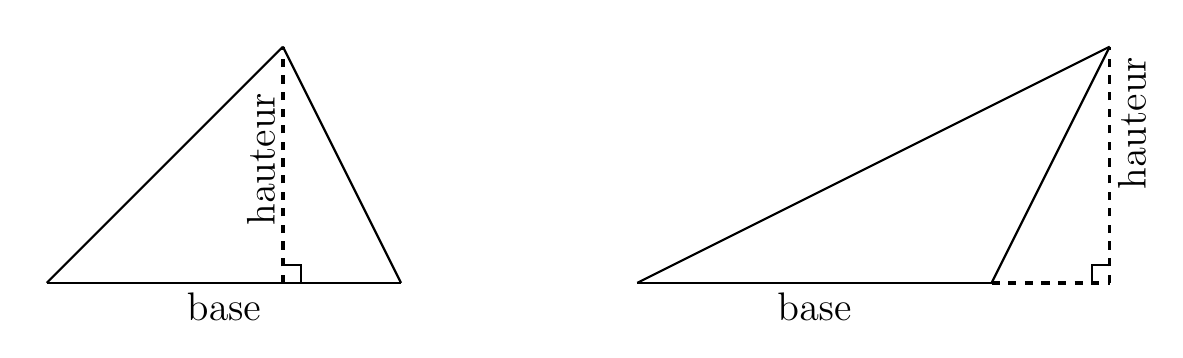
\begin{tikzpicture}[scale=1.5]
		\draw[-, thick, black] (0,0) -- (3,0) node[midway, below] {base};
		\draw[-, thick, black] (3,0) -- (2,2);
		\draw[-, thick, black] (2,2) -- (0,0);
		
		\node[black, left] at  (0,0) {};
		\node[black, below] at  (2,0) {};
		\node[black, above] at  (2,2) {};
		
		% angle droit
		\draw[-, thick, black] (2,.15)-- (2.15,.15) -- (2.15,0);
		
		%hauteur
		\draw[-,very thick, black, dashed] (2,0) -- (2,2) node[pos=.85, left=8pt, rotate=90] {hauteur};
		
		\draw[-, thick, black] (5,0) -- (8,0) node[midway, below] {base};
		\draw[-, thick, black] (8,0) -- (9,2);
		\draw[-, thick, black] (9,2) -- (5,0);
		
		\node[black, left] at  (5,0) {};
		\node[black, below] at  (9,0) {};
		\node[black, above] at  (9,2) {};
		
		% droite base
		\draw[-, very thick, black, dashed] (8,0) -- (9,0);
		
		% angle droit
		\draw[-, thick, black] (9,.15)-- (8.85,.15) -- (8.85,0);
		
		%hauteur
		\draw[-, very thick, black, dashed] (9,0) -- (9,2) node[pos=.35, right=8pt, rotate=90] {hauteur};
	\end{tikzpicture}
	
	% page 2
	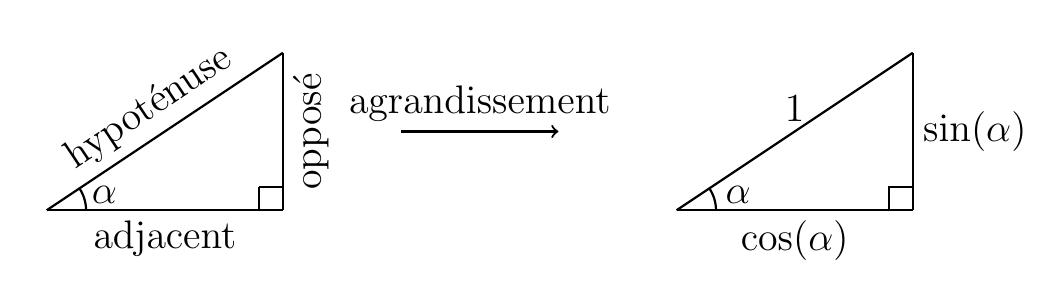
\begin{tikzpicture}[scale=1]
		\draw[-, thick, black] (0,0) -- (3,0) node[midway, below] {adjacent};
		\draw[-, thick, black] (3,0) -- (3,2) node[midway, below, rotate=90] {opposé};
		\draw[-, thick, black] (3,2) -- (0,0) node[midway, rotate=33.69, above]{hypoténuse};
		
		\node[black, left] at  (0,0) {};
		\node[black, below] at  (3,0) {};
		\node[black, above] at  (3,2) {};
		% angle droit
		\draw[-, thick, black] (3,.3)-- (2.7,.3);
		\draw[-, thick, black] (2.7,.3)-- (2.7,0);
		
		% angle
		\draw [black,thick,domain=0:35] plot ({.5*cos(\x)}, {.5*sin(\x)});
		\node[black, right] at  (0.45,.2) {$\alpha$};
		
		% %
		
		\draw[->, thick, black] (4.5,1) -- (6.5,1) node[midway, above]{agrandissement};
	
		\draw[-, thick, black] (8,0) -- (11,0) node[midway, below] {$\cos(\alpha)$};
		\draw[-, thick, black] (11,0) -- (11,2)node[midway, right] {$\sin(\alpha)$};
		\draw[-, thick, black] (11,2) -- (8,0) node[midway, above]{1};
		
		\node[black, left] at  (8,0) {};
		\node[black, below] at  (11,0) {};
		\node[black, above] at  (11,2) {};
		% angle droit
		\draw[-, thick, black] (11,.3)-- (10.7,.3) -- (10.7,0);
		
		% angle
		\draw [black,thick,domain=0:35] plot ({8+.5*cos(\x)}, {.5*sin(\x)});
		\node[black, right] at  (8.5,.2) {$\alpha$};
		
	\end{tikzpicture}
	
	% page 3
	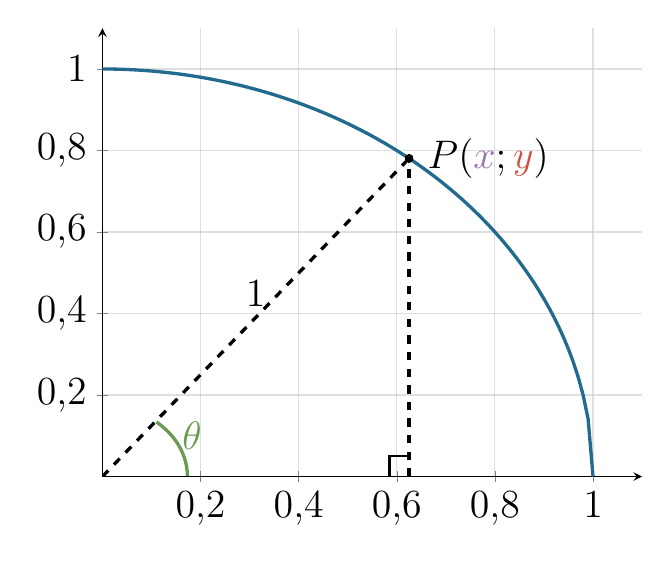
\begin{tikzpicture}[>=stealth, scale=1]
		\begin{axis}[xmin = 0, xmax=1.1, ymin=0, ymax=1.1, axis x line=middle, axis y line=middle, axis line style=->, grid=both, grid style = {opacity=.5}]
			\addplot[no marks, BLUE_E, -, very thick] expression[domain=0:1, samples=101]{sqrt(1-x^2)};
			\addplot[mark=*, mark size = 1, black, thick] (0.625, 0.7805) node[right=3pt] {$P({\color{PURPLE}x};{\color{RED_E}y})$};
			
			
			\addplot[black, dashed, very thick] expression[domain=0:0.625, samples=2]{0.7805/0.625*x}
			node[midway, above=]{$1$};
			
			\addplot[no marks, GREEN_E, -, very thick] expression[domain=0.11:0.1732, samples=101]{sqrt(.03-x^2)}
			node[right, pos=.3] {$\theta$};
			
			\draw[black, dashed, very thick] (axis cs:0.625, 0) -- (axis cs:0.625,0.7805);
			
			% angle droit
			\draw[-, thick, black] (axis cs:0.585,0) -- (axis cs:0.585,.05) -- (axis cs:0.625,.05);
		\end{axis}
	\end{tikzpicture}
	
	% pages 4-5-6-7
	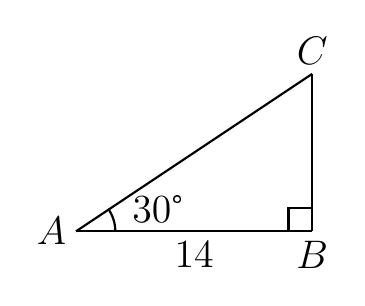
\begin{tikzpicture}[scale=1]
		\draw[-, thick, black] (0,0) -- (3,0) node[midway, below] {$14$};
		\draw[-, thick, black] (3,0) -- (3,2);
		\draw[-, thick, black] (3,2) -- (0,0);
		
		\node[black, left] at  (0,0) {$A$};
		\node[black, below] at  (3,0) {$B$};
		\node[black, above] at  (3,2) {$C$};
		% angle droit
		\draw[-, thick, black] (3,.3)-- (2.7,.3) -- (2.7,0);
		
		% angle
		\draw [black,thick,domain=0:35] plot ({.5*cos(\x)}, {.5*sin(\x)})
		node[left=5pt, right=5pt] {$30$°};
	\end{tikzpicture}
	
	
	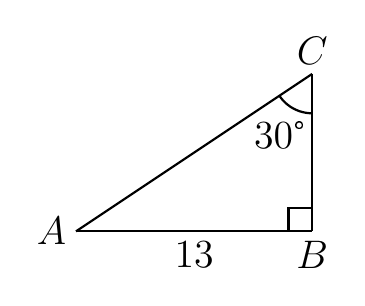
\begin{tikzpicture}[scale=1]
		\draw[-, thick, black] (0,0) -- (3,0) node[midway, below] {$13$};
		\draw[-, thick, black] (3,0) -- (3,2);
		\draw[-, thick, black] (3,2) -- (0,0);
		
		\node[black, left] at  (0,0) {$A$};
		\node[black, below] at  (3,0) {$B$};
		\node[black, above] at  (3,2) {$C$};
		% angle droit
		\draw[-, thick, black] (3,.3)-- (2.7,.3) -- (2.7,0);
		
		% angle
		\draw [black,thick,domain=270:215] plot ({3+.5*cos(\x)}, {2+.5*sin(\x)})
		node[below=5pt] {$30$°};
	\end{tikzpicture}
	

	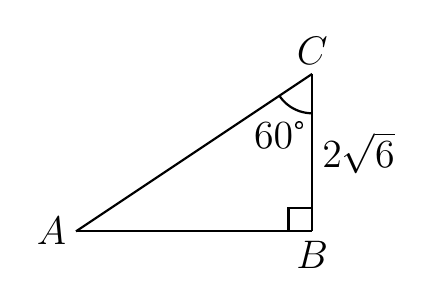
\begin{tikzpicture}[scale=1]
		\draw[-, thick, black] (0,0) -- (3,0);
		\draw[-, thick, black] (3,0) -- (3,2) node[midway, right] {$2\sqrt{6}$} ;
		\draw[-, thick, black] (3,2) -- (0,0);
		
		\node[black, left] at  (0,0) {$A$};
		\node[black, below] at  (3,0) {$B$};
		\node[black, above] at  (3,2) {$C$};
		% angle droit
		\draw[-, thick, black] (3,.3)-- (2.7,.3) -- (2.7,0);
		
		% angle
		\draw [black,thick,domain=270:215] plot ({3+.5*cos(\x)}, {2+.5*sin(\x)})
		node[below=5pt] {$60$°};
	\end{tikzpicture}



	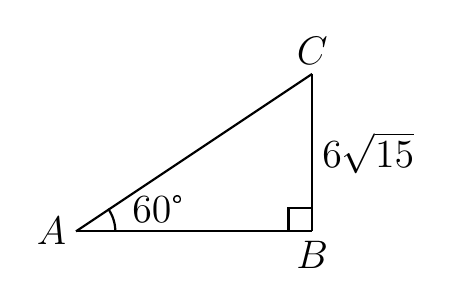
\begin{tikzpicture}[scale=1]
		\draw[-, thick, black] (0,0) -- (3,0);
		\draw[-, thick, black] (3,0) -- (3,2)  node[midway, right] {$6\sqrt{15}$} ;
		\draw[-, thick, black] (3,2) -- (0,0);
		
		\node[black, left] at  (0,0) {$A$};
		\node[black, below] at  (3,0) {$B$};
		\node[black, above] at  (3,2) {$C$};
		% angle droit
		\draw[-, thick, black] (3,.3)-- (2.7,.3) -- (2.7,0);
		
		% angle
		\draw [black,thick,domain=0:35] plot ({.5*cos(\x)}, {.5*sin(\x)})
		node[left=5pt, right=5pt] {$60$°};
	\end{tikzpicture}
	
	% page 8
	\begin{tikzpicture}[scale=.8]
		\draw[-, thick, black] (0,0) -- (10, 4) node[below]{$(d)$};
	
		\node[black] at (7,0){$\bullet$};
		\node[right, GREEN_E] at (7,0) {$M$};
		
		\node[black] at (70*10/116,70*4/116 - .03) {$\bullet$};
		\node[above, BLUE_E] at  (70*10/116,70*4/116) {$M'$};
		
		% proj pourquoi ai-je calculé ça
		\draw[-, very thick, black, dashed] (7,0) -- (70*10/116,70*4/116);
		% angle droit à vue d'oeil car y'en a marre
		\draw[-, thick, black] (70*10/116*0.95, 70*4/116*0.95) -- (5.87,2)  -- (6.15,2.1);
	\end{tikzpicture}
	
	% page 9
	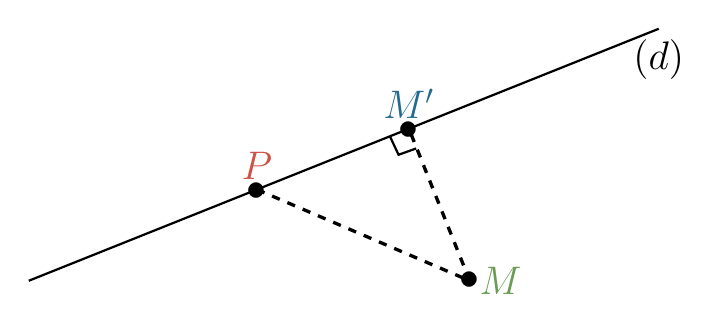
\begin{tikzpicture}[scale=.8]
		\draw[-, thick, black] (0,0) -- (10, 4) node[below]{$(d)$};
	
		\node[black] at (7,0){$\bullet$};
		\node[black, right, GREEN_E] at (7,0) {$M$};
		
		\node[black] at (70*10/116 ,70*4/116 - .03) {$\bullet$};
		\node[black, above, BLUE_E] at  (70*10/116,70*4/116) {$M'$};
		
		\draw[-, very thick, black, dashed] (7,0) -- (70*10/116,70*4/116);
		\draw[-, thick, black] (70*10/116*0.95, 70*4/116*0.95) -- (5.87,2) -- (6.15,2.1);
	
	
		\node[black] at (70*10/116*.6,70*4/116*.6-.03) {$\bullet$};
		\node[black, above, RED_E] at  (70*10/116*.6,70*4/116*.6) {$P$};
		\draw[-, very thick, black, dashed] (70*10/116*.6,70*4/116*.6) -- (7,0);
	\end{tikzpicture}
	
	% page 10
	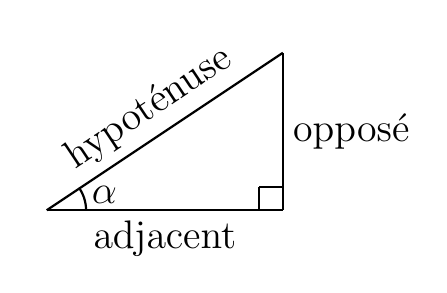
\begin{tikzpicture}[scale=1]
		\draw[-, thick, black] (0,0) -- (3,0) node[midway, below] {adjacent};
		\draw[-, thick, black] (3,0) -- (3,2) node[midway, right] {opposé};
		\draw[-, thick, black] (3,2) -- (0,0) node[midway, rotate=33.69, above]{hypoténuse};
		
		\node[black, left] at  (0,0) {};
		\node[black, below] at  (3,0) {};
		\node[black, above] at  (3,2) {};
		% angle droit
		\draw[-, thick, black] (3,.3)-- (2.7,.3);
		\draw[-, thick, black] (2.7,.3)-- (2.7,0);
		
		% angle
		\draw [black,thick,domain=0:35] plot ({.5*cos(\x)}, {.5*sin(\x)});
		\node[black, right] at  (0.45,.2) {$\alpha$};
	\end{tikzpicture}
	% page 11
	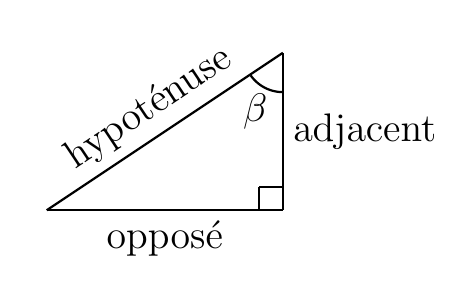
\begin{tikzpicture}[scale=1]
		\draw[-, thick, black] (0,0) -- (3,0) node[midway, below] {opposé};
		\draw[-, thick, black] (3,0) -- (3,2) node[midway, right] {adjacent};
		\draw[-, thick, black] (3,2) -- (0,0) node[midway, rotate=33.69, above]{hypoténuse};
		
		\node[black, left] at  (0,0) {};
		\node[black, below] at  (3,0) {};
		\node[black, above] at  (3,2) {};
		% angle droit
		\draw[-, thick, black] (3,.3)-- (2.7,.3);
		\draw[-, thick, black] (2.7,.3)-- (2.7,0);
		
		% angle
		\draw [black,thick,domain=215:270] plot ({3+.5*cos(\x)}, {2+.5*sin(\x)});
		\node[black, below] at  (2.65,1.6) {$\beta$};
	\end{tikzpicture}
	
	% page 12
	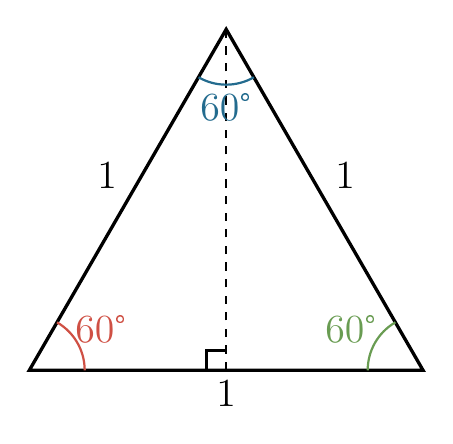
\begin{tikzpicture}[scale=5]
	\draw[-, thick, dashed] (.5,0) -- (.5, .866);
	
	
	\draw[-, very thick] 
	(0,0) coordinate (A) -- 
	(1,0) coordinate (B) node[midway, below] {1} -- 
	(.5, .866)  coordinate (C) node[midway, above right] {1} -- 
	cycle node[midway, above left] {1} 
	pic ["60°", draw,-,RED_E,thick,angle radius=20pt, angle eccentricity=1.5] {angle = B--A--C}
	pic ["60°", draw,-,GREEN_E,thick,angle radius=20pt, angle eccentricity=1.5] {angle = C--B--A}
	pic ["60°", draw,-,BLUE_E,thick,angle radius=20pt, angle eccentricity=1.4] {angle = A--C--B};
	
	
	\draw[-, thick] (.45,0) -- (.45, .05) -- (.5, .05);
	\end{tikzpicture}
	
	% page 13
	\begin{tikzpicture}[scale=5]
	
	\draw[-, very thick] 
	(0,0) coordinate (A) -- 
	(.5,0) coordinate (B) node[midway, below] {$1/2$} -- 
	(.5, .866)  coordinate (C) node[midway, right] {$h = \dfrac{\sqrt3}2$} -- 
	cycle node[midway, above left] {1} 
	pic ["60°", draw,-,RED_E,thick,angle radius=20pt, angle eccentricity=1.5] {angle = B--A--C}
	pic ["30°", draw,-,BLUE_E,thick,angle radius=40pt, angle eccentricity=1.25] {angle = A--C--B};
	
	\draw[-, thick] (.45,0) -- (.45, .05) -- (.5, .05);
	\end{tikzpicture}
	
	% page 14
	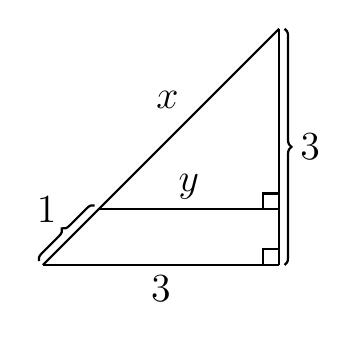
\begin{tikzpicture}[scale=1]
	\draw[-, thick] 
	(0,0) -- (3,0) node[midway, below] {$3$};
	\draw[-, thick] 
	(3,0) -- (3, 3);
	\draw[-, thick, decorate, decoration={brace, raise=2pt, mirror}] 
	(3,0) -- (3, 3) node[midway, right=4pt] {$3$};
	\draw[-, thick] 
	(0,0) -- (0.707, 0.707);
	\draw[-, thick, decorate, decoration={brace, raise=2pt}] 
	(0,0) -- (0.707, 0.707) node[midway, above left=2pt] {$1$};
	\draw[-, thick] 
	 (0.707, 0.707) -- (3,3) node[midway, above left] {$x$};
	\draw[-, thick] 
	 (0.707, 0.707) -- (3,.707) node[midway, above] {$y$};
	
	\draw[-, thick] (2.8,0) -- (2.8, .2) -- (3, .2);
	\draw[-, thick] (2.8,0.707) -- (2.8, .907) -- (3, .907);
	\end{tikzpicture}
	
	% page 15
	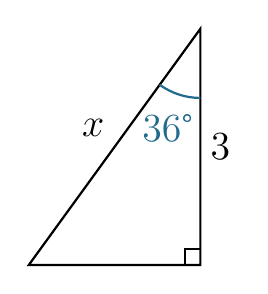
\begin{tikzpicture}[scale=1]
	\draw[-, thick] 
	(0,0) coordinate (A) -- 
	(2.179,0) coordinate (B) -- 
	(2.179,3)  coordinate (C) node[midway, right] {$3$} -- 
	cycle node[midway, above left] {$x$} 
	pic ["36°", draw,-,BLUE_E,thick,angle radius=25pt, angle eccentricity=1.5] {angle = A--C--B};
	
	\draw[-, thick] (1.979,0) -- (1.979, .2) -- (2.179, .2);
	\end{tikzpicture}
	
	% page 16
	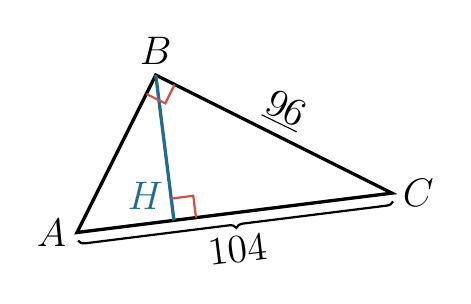
\begin{tikzpicture}[scale=1]
	
	% triangle
	\draw[-, very thick] (0,0) coordinate (A) node[left]{$A$}
		-- (4, .5) coordinate (C) node[right]{$C$}
		-- (1,2) coordinate (B) node[above]{$B$}
		-- cycle;
	
	\draw[- , thick, decorate, decoration = {brace, mirror, raise=3pt}] (A) -- (C) node[midway,below=5pt,rotate=7]{104};
	\draw[- , thick] (B)--(C) node[midway,above,rotate=-26]{\underline{96}};
	
	%hauteur
	\draw[-, very thick, BLUE_E] (B) -- (80/65, 10/65) coordinate (H) node[above left] {$H$}; 
	
	% angles droits
	\draw[-, thick, RED_E] ($(H)+.07*(C)$) -- ($(H)+.07*(C) + .15*(B)-.15*(H)$) -- ($(H) + .15*(B)-.15*(H)$) ;
	
	\draw[-, thick, RED_E] ($(B) + .08*(C) - .08*(B)$) -- ($(B) + .08*(C) - .08*(B) - .12*(B)$) -- ($(B) - .12*(B)$) ;
	
	\end{tikzpicture}
	
	% page 17
	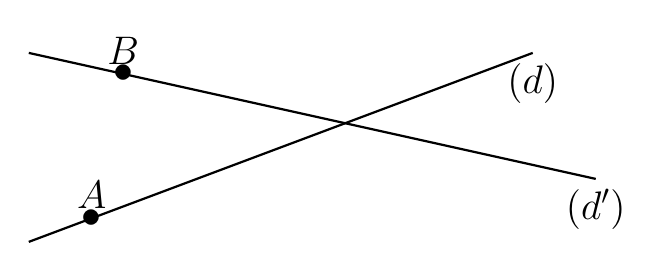
\begin{tikzpicture}[scale=.8]
		\draw[-, thick, black] (0,0) -- (8, 3) node[below]{$(d)$};
		\draw[-, thick, black] (0,3) -- (9, 1) node[below]{$(d')$};
	
		\node[black] at (1, 3/8) {$\bullet$};
		\node[black, above] at (1, 3/8) {$A$};
		
		\node[black] at (1.5, 24/9) {$\bullet$};
		\node[black, above] at  (1.5, 24/9) {$B$};
	\end{tikzpicture}
	
	% page 18
	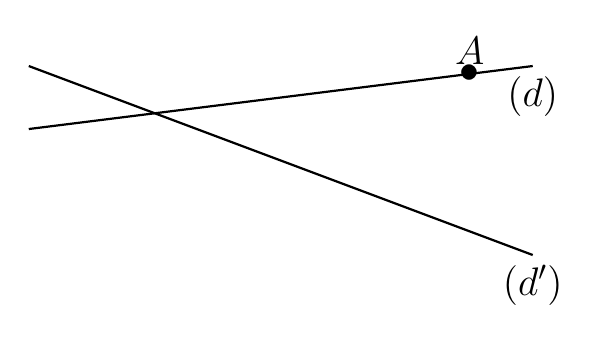
\begin{tikzpicture}[scale=.8]
		\draw[-, thick, black] (0,0) -- (8, 1) node[below]{$(d)$};
		\draw[-, thick, black] (0,1) -- (8, -2) node[below]{$(d')$};
	
		\node[black] at (7, 7/8) {$\bullet$};
		\node[black, above] at  (7, 7/8)  {$A$};
	\end{tikzpicture}
	
	% page 19
	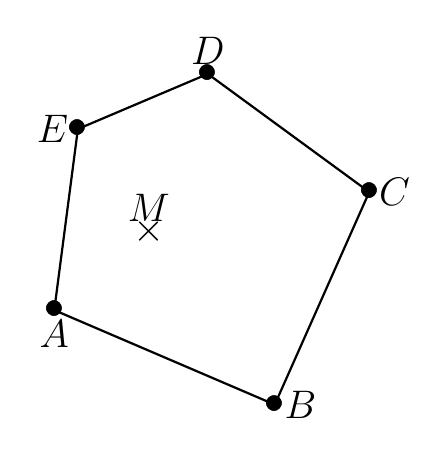
\begin{tikzpicture}
		\draw[-, thick, black] (0,0) node{$\bullet$} -- (2.8, -1.2) node{$\bullet$};
		\draw[-, thick, black] (2.8,-1.2) node{$\bullet$} -- (4, 1.5) node{$\bullet$};
		\draw[-, thick, black] (4, 1.5) node{$\bullet$} -- (1.95,3) node{$\bullet$};
		\draw[-, thick, black] (1.95,3) node{$\bullet$} -- (.3,2.3)  node{$\bullet$};
		\draw[-, thick, black] (.3,2.3) node{$\bullet$} -- (0,0) node{$\bullet$};
		
		\node[black, below] at  (0,0)  {$A$};
		\node[black, right] at  (2.8,-1.2)  {$B$};
		\node[black, right] at  (4, 1.5)  {$C$};
		\node[black, above] at  (1.95,3)  {$D$};
		\node[black, left] at (.3,2.3)  {$E$};
		
		
		\node[black, above] at (1.2, 1) {$M$};
		\node[black] at (1.2, 1) {$\times$};
	
	\end{tikzpicture}
	
	% page 20
	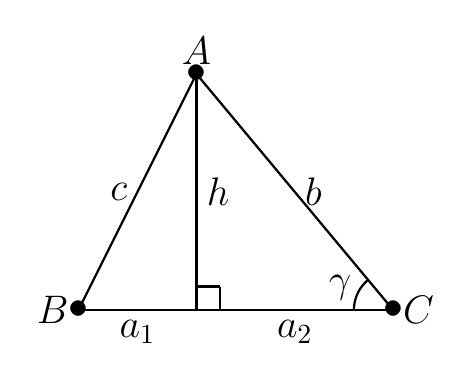
\begin{tikzpicture}[scale=1]
		\draw[-, thick, black] (0,0) node{$\bullet$} -- (1.5,0) node[midway, below] {$a_1$};
		\draw[-, thick, black] (1.5,0) -- (4,0) node[midway, below] {$a_2$};
		\draw[-, thick, black] (4, 0) node{$\bullet$} -- (1.5,3) node[midway, right] {$b$};
		\draw[-, thick, black] (1.5,3) node{$\bullet$}-- (0,0) node[midway, left] {$c$};
		
		\node[black, left] at  (0,0) {$B$};
		\node[black, right] at  (4,0) {$C$};
		\node[black, above] at  (1.5,3) {$A$};
		
		\draw[-, thick, black] (1.5,0)-- (1.5,3) node[midway, right] {$h$};
		
		% angle droit
		\draw[-, thick, black] (1.5,.3)-- (1.8,.3);
		\draw[-, thick, black] (1.8,.3)-- (1.8,0);
		
		% angle
		\draw [black,thick,domain=130:180] plot ({4+.5*cos(\x)}, {.5*sin(\x)})
		node[left=5pt, above] {$\gamma$};
	\end{tikzpicture}
	
	% page 21
	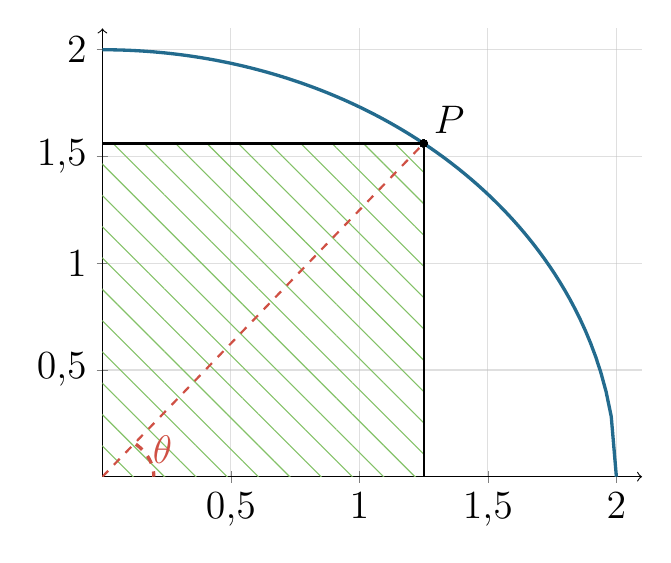
\begin{tikzpicture}[scale=1]
		\begin{axis}[xmin = 0, xmax=2.1, ymin=0, ymax=2.1, axis x line=middle, axis y line=middle, axis line style=->, grid=both]
		
			\draw[draw=none, pattern={Lines[angle=-45,distance=8pt]}, pattern color=GREEN] (axis cs:0,0) rectangle ++(axis cs:1.25,1.561);
		
			\addplot[no marks, BLUE_E, -, very thick] expression[domain=0:2, samples=101]{sqrt(4-x^2)};
			\addplot[black, mark=*, mark size = 1, thick] (1.25, 1.561) node[above right] {$P$};
			
			
			\addplot[-, thick, dashed, RED_E] expression[domain=0:1.25, samples=2]{1.561/1.25*x};
			
			\addplot[RED_E, -, very thick, dashed] expression[domain=0.13:.2, samples=101]{sqrt(.04-x^2)}
			node[right, pos=.2] {$\theta$};
			
			\addplot[black, -, thick] expression[domain=0:1.25, samples=2]{1.561};
			\draw[black, thick] (axis cs:1.25, 0) -- (axis cs:1.25,1.561);
		\end{axis}
	\end{tikzpicture}
	
	% page 22
	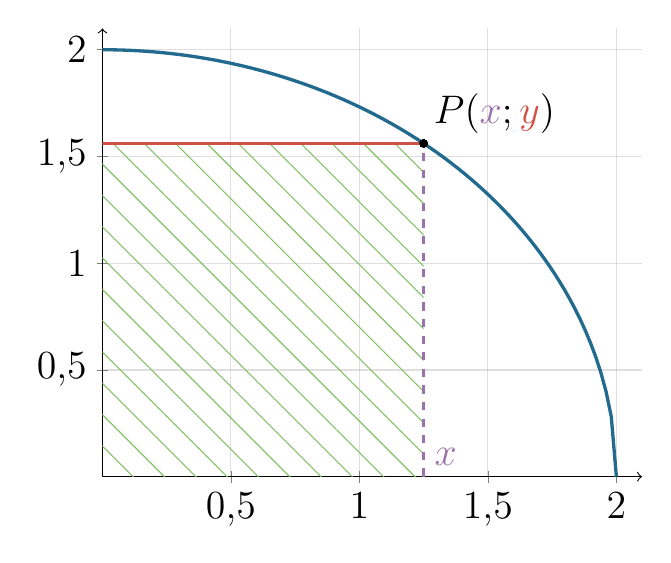
\begin{tikzpicture}[scale=1]
		\begin{axis}[xmin = 0, xmax=2.1, ymin=0, ymax=2.1, axis x line=middle, axis y line=middle, axis line style=->, grid=both]
		
			\draw[draw=none,pattern={Lines[angle=-45,distance=8pt]}, pattern color=GREEN] (axis cs:0,0) rectangle ++(axis cs:1.25,1.561);
			
			\addplot[no marks, BLUE_E, -, very thick] expression[domain=0:2, samples=101]{sqrt(4-x^2)};
			\addplot[black, mark=*, mark size = 1, thick] (1.25, 1.561) node[above right] {$P({\color{PURPLE}x};{\color{RED_E}y})$};
			
			\addplot[RED_E, -, thick] expression[domain=0:1.25, samples=2]{1.561};
			\draw[very thick, dashed, PURPLE] (axis cs:1.25, 0) -- (axis cs:1.25,1.561)
			node[above right, pos=0] {$x$};
		\end{axis}
	\end{tikzpicture}
	
	% page 23
	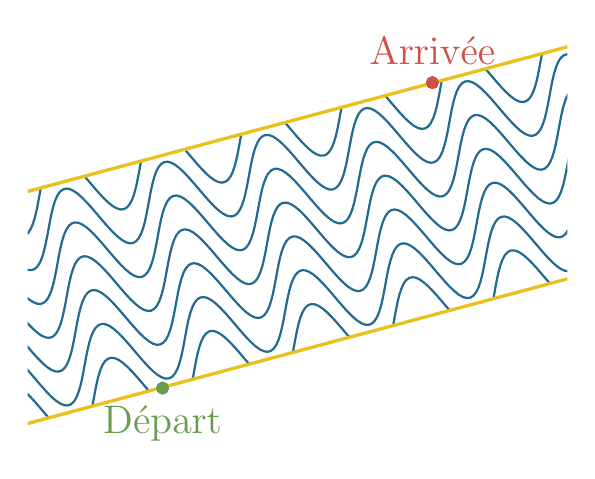
\begin{tikzpicture}[scale=1]
		\begin{axis}[xmin = 0, xmax=8, ymin=-.5, ymax=1.1,
		axis x line=none, axis y line=none, 
		grid=none,
		]
			\begin{scope}
			\clip[rotate=15] (axis cs:0,-.4) rectangle (axis cs:10,.4);
			\foreach \i in {-3, -2, -1, ..., 3}
				\addplot[no marks, BLUE_E, -, thick, rotate=15] expression[domain=0:10, samples=200]{cos(x*180*1.3)/8+\i/8};
			\end{scope}
			
			\draw[very thick, YELLOW_E, rotate=15] (axis cs:0,-.4) rectangle (axis cs:10,.4);
				
			\addplot[mark=*, mark size=2pt, GREEN_E] (2,-.27) node[below=3pt]{Départ};
			\addplot[mark=*, mark size=2pt, RED_E] (6,.82) node[above=3pt]{Arrivée};
		\end{axis}
	\end{tikzpicture}
%
\end{document}